\subsection{miniWECC-genTrip - WIP} 
Shows multi generator tripping, use of miniWECC in all versions.

Difference between 3.1 and 4: speed, zeroing of tripped machine derivative, system inertia calculation.\\
3.1: 110.0729 seconds\\
4.0: 46.3361 seconds\\
2.37 x Speed up in PST 4

Version 3 does not zero derivatives of tripped machine speeds.
\begin{figure}[H]
	\centering
	\footnotesize
	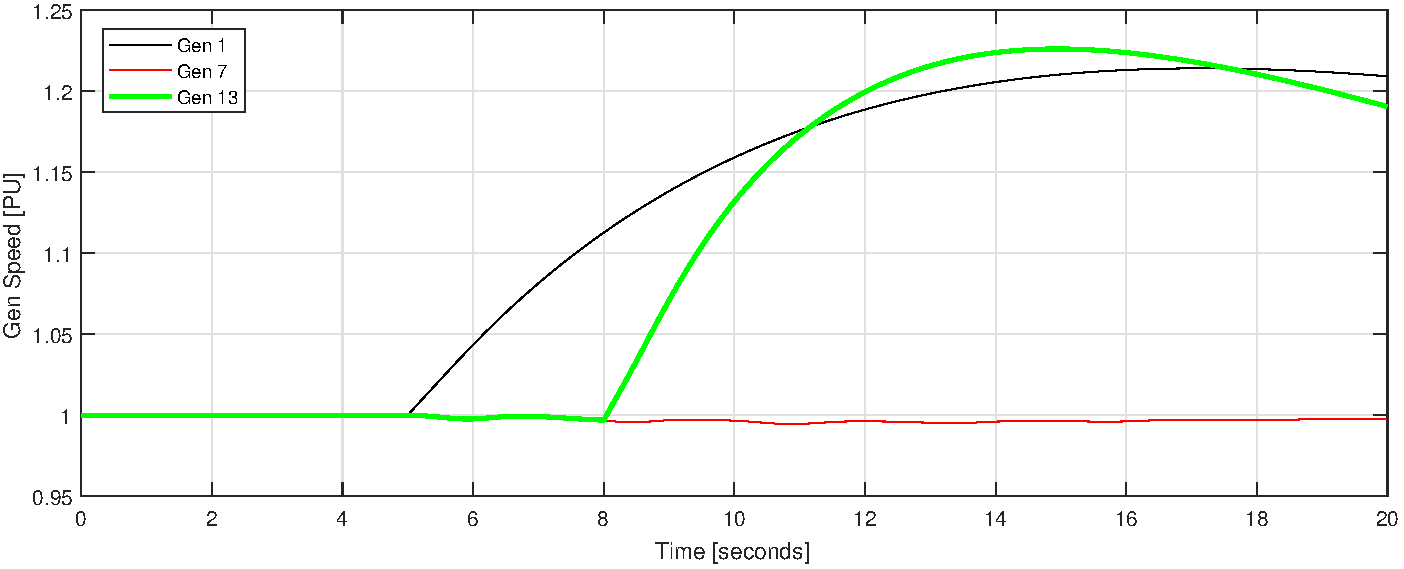
\includegraphics[width=\linewidth]{examples/miniWECC/mwGenTrip-3-Speed}
	\caption{Select generator speed during PST 3.1 run\_mwGenTrip.}
	\label{fig: mwGenTrip 3 speed}
\end{figure}%\vspace{-1 em}

\pagebreak
PST 4 zeros derivatives of tripped machine speed and calculates system inertia accounting for tripped machines.
\begin{figure}[H]
	\centering
	\footnotesize
	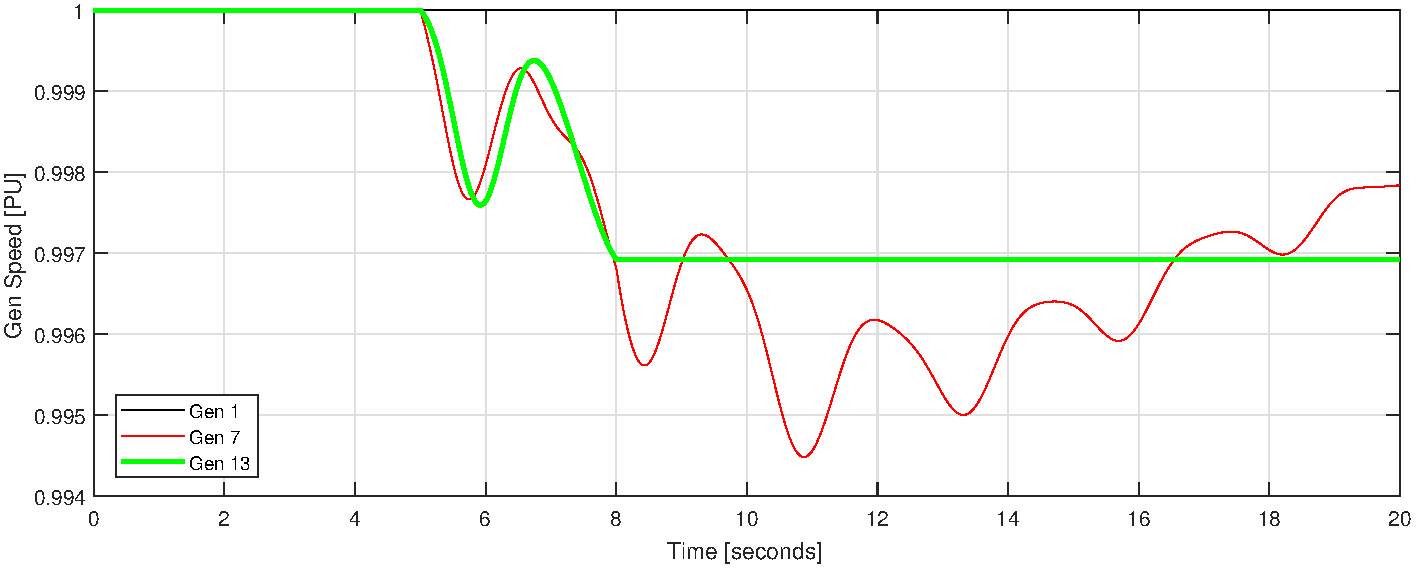
\includegraphics[width=\linewidth]{examples/miniWECC/mwGenTrip-4-Speed}
	\caption{Select generator speed during PST 4.0 run\_mwGenTrip.}
	\label{fig: mwGenTrip 4 speed}
\end{figure}%\vspace{-1 em}

\begin{figure}[H]
	\centering
	\footnotesize
	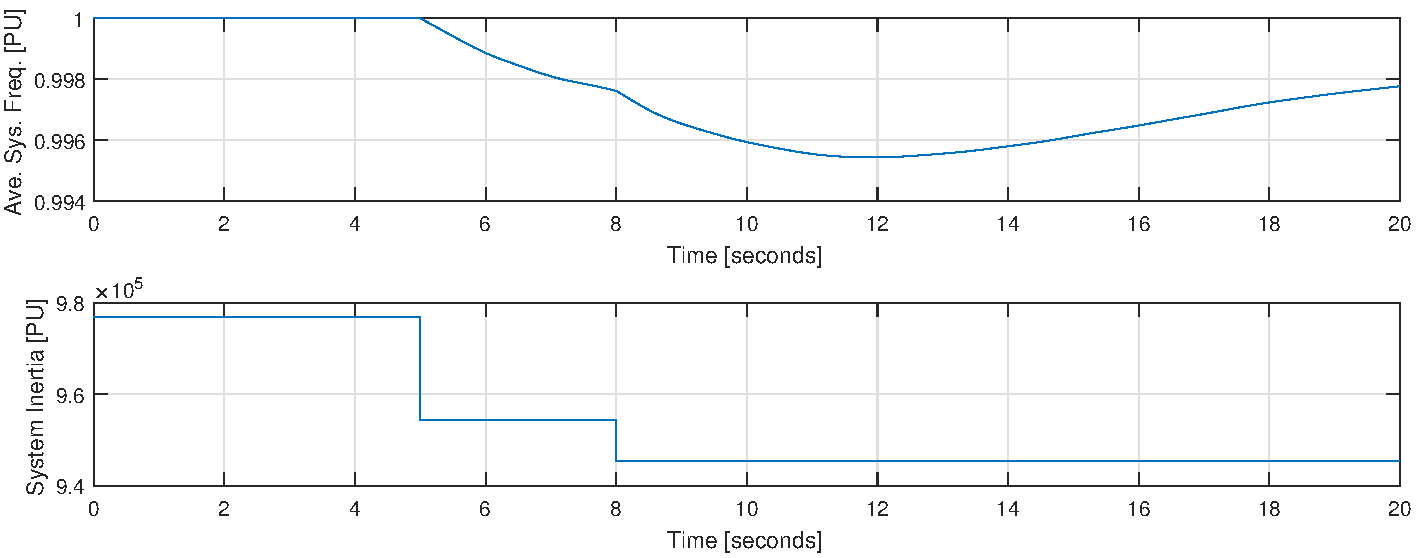
\includegraphics[width=\linewidth]{examples/miniWECC/mwGenTrip-4-FandH}
	\caption{Calculated system inertia during PST 4.0 run\_mwGenTrip.}
	\label{fig: mwGenTrip 4 FandH}
\end{figure}%\vspace{-1 em}